\documentclass[lettersize,journal]{IEEEtran}
\usepackage{amsmath,amsfonts}
\usepackage{array}
\usepackage[caption=false,font=normalsize,labelfont=sf,textfont=sf]{subfig}
\usepackage{textcomp}
\usepackage{stfloats}
\usepackage{url}
\usepackage{graphicx}
\usepackage{cite}
\usepackage{tikz}
\usetikzlibrary{arrows.meta,positioning}
\hyphenation{op-tical net-works semi-conduc-tor IEEE-Xplore}

\newcommand{\safeimg}[3][4.5cm]{%
 \IfFileExists{#3}{\includegraphics[width=#2,height=#1,keepaspectratio]{#3}}%
 {\fbox{\parbox[c][2.4cm][c]{\dimexpr#2-2\fboxsep-2\fboxrule\relax}%
 {\centering\scriptsize Missing file:\\\texttt{\detokenize{#3}}}}}}

\begin{document}

\title{Digital Image Processing for Real-World Cases:\\ A Review of Suitable Features}

\author{Nabila Aisy Shifa,~NIM~25/560484/PA/23619
\thanks{Course assignment, Digital Image Processing, Universitas Gadjah Mada (UGM), Yogyakarta, Indonesia.}
\thanks{Manuscript prepared in November 2026.}}

\markboth{Pengolahan Citra Digital -- Course Report, November 2026}%
{Digital Image Processing -- Course Report}

\maketitle

\begin{abstract}
This report summarizes four real-world problems that can be solved with digital image processing: ripeness grading of oil palm fruit bunches, lane marking detection, license plate recognition, and blood cell counting. For each case, one representative open paper is reviewed, its processing pipeline is outlined, and the image features that suit the problem are identified and justified. The cases show that the feature should follow the cue that actually separates the classes: color for ripeness grading, edges and straight lines for lane markings, vertical edges and geometric shape for license plates, and circularity and size for blood cells.
\end{abstract}

\begin{IEEEkeywords}
Digital image processing, feature extraction, color features, edge detection, Hough transform, morphology.
\end{IEEEkeywords}

\section{Introduction}
\IEEEPARstart{D}{igital} image processing (DIP) turns raw pixels into information that a computer can act on. A typical solution follows the chain in Fig.~\ref{fig:pipeline}: an image is acquired, enhanced, segmented, described by features, and finally used for a decision such as classifying, counting, or locating objects \cite{gw}. The step that connects pixels to a decision is feature extraction. A feature is a compact measurement, such as color statistics, edge strength, line parameters, or shape descriptors, that separates the classes of interest. A feature that suits one problem can be useless in another, so the key design question is which feature captures what actually differs between the classes.

This report reviews four cases and, for each one, identifies the suitable features and explains why they fit.

\begin{figure}[!t]
\centering
\resizebox{\columnwidth}{!}{%
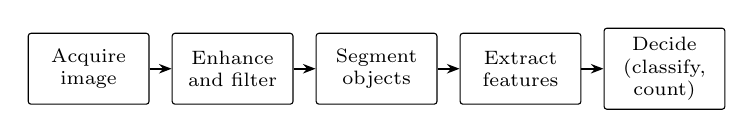
\begin{tikzpicture}[node distance=0.28cm,
 box/.style={draw,rounded corners=1pt,align=center,font=\scriptsize,minimum height=0.9cm,text width=1.3cm},
 arr/.style={-{Stealth[length=1.6mm]},thick}]
\node[box] (a) {Acquire\\image};
\node[box,right=of a] (b) {Enhance\\and filter};
\node[box,right=of b] (c) {Segment\\objects};
\node[box,right=of c] (d) {Extract\\features};
\node[box,right=of d] (e) {Decide\\(classify, count)};
\draw[arr] (a)--(b);
\draw[arr] (b)--(c);
\draw[arr] (c)--(d);
\draw[arr] (d)--(e);
\end{tikzpicture}}
\caption{General digital image processing pipeline used by all four cases.}
\label{fig:pipeline}
\end{figure}

\section{Case Studies}

\subsection{Oil Palm Ripeness Grading: Color Features}
\textit{Problem.} The ripeness of oil palm fruit bunches affects oil quality, yet manual grading depends on subjective visual judgment. Zulkhoiri \textit{et al.} \cite{palm} classify bunches as ripe, half-ripe, or unripe from photographs.

\textit{Pipeline.} The dataset has 257 images (100 ripe, 101 half-ripe, 57 unripe). Each image is cropped to the bunch region and resized from 9000$\times$12000 to 300$\times$400 pixels. The image is converted to HSV, RGB, and YCbCr, and the mean and standard deviation of every channel form the feature vector, which is classified by k-NN and SVM.

\textit{Suitable features.} Ripening changes the skin color of the bunch, while its shape and size hardly change, so color statistics capture the discriminating cue directly. Chromatic channels (H in HSV, Cb and Cr in YCbCr) are separated from brightness, which reduces sensitivity to lighting \cite{palm}. YCbCr with k-NN reached 97.40\% (hold-out) and YCbCr with SVM reached 100\% (10-fold). RGB with SVM also reached 100\%, so the gain comes from color information itself rather than from one ``best'' color space. The unripe class is the hardest for k-NN (68.8\% recall with HSV) because its colors overlap with ripe bunches. A limitation is that all images come from one plantation.

\begin{figure}[!t]
\centering
\safeimg{\columnwidth}{fig_palm.png}
\caption{Example oil palm fruit bunch images: (a) unripe, (b) ripe, and (c) half-ripe. Reproduced from \cite{palm}, CC BY 4.0.}
\label{fig:palm}
\end{figure}

\subsection{Lane Marking Detection: Edge and Line Features}
\textit{Problem.} Lane detection supports driver assistance and autonomous driving. Javeed \textit{et al.} \cite{lane} propose a classical pipeline for complex road conditions.

\textit{Pipeline.} The frame is converted to grayscale and smoothed with a Gaussian filter. A Sobel gradient, non-maximum suppression, Otsu thresholding \cite{otsu}, and Canny edge detection \cite{canny} follow. A triangular region of interest covers the lower part of the image, and a fast Hough transform \cite{hough} finds straight lines. Left and right lanes are separated by line slope.

\textit{Suitable features.} Lane paint is a bright, elongated strip with strong contrast against asphalt, so it appears as strong intensity gradients (edge feature) that lie along straight lines (line feature). The Hough transform lets each edge pixel vote in the $(\rho,\theta)$ parameter space, where every straight lane becomes a peak, so broken or partly hidden markings can still be recovered. On 160 TuSimple images the method reached a maximum accuracy of 96.7\% at 22.2~ms per frame. It detects only straight lines, is sensitive to threshold parameters, and struggles with faint markings \cite{lane}.

\begin{figure}[!t]
\centering
\subfloat[]{\safeimg{0.47\columnwidth}{fig_lane_roi.png}\label{fig:lane_a}}
\hfil
\subfloat[]{\safeimg{0.47\columnwidth}{fig_lane_result.png}\label{fig:lane_b}}
\caption{Lane detection with the fast Hough transform: (a) edge detection and road region of interest, (b) detection results on TuSimple frames. Adapted from \cite{lane}, CC BY.}
\label{fig:lane}
\end{figure}

\subsection{License Plate Recognition: Edge and Shape Features}
\textit{Problem.} Automatic plate recognition supports traffic monitoring and parking management. Azad \textit{et al.} \cite{plate} target plates that are tilted and images of poor quality.

\textit{Pipeline.} The image is converted to grayscale, smoothed, and binarized with a threshold equal to the mean plus the variance of the gray image. Sobel vertical edges are extracted, and erosion followed by dilation merges the characters into one compact region. Candidates are filtered by geometric ratio, and plate tilt is corrected. Characters are segmented by labeling, thinned to a skeleton, and split into 18 frames of 10$\times$10 pixels. Each frame contributes a mean distance and a mean angle, and k-NN recognizes the character.

\textit{Suitable features.} The strokes of letters and digits create a dense cluster of vertical edges inside a rectangular region, so vertical-edge density locates the plate and geometric constraints (extent and aspect ratio) validate it. Skeleton-based distance and angle features then describe character shape. On 100 phone-camera images, 98 plates were localized and 792 of 800 characters (99.12\%) were recognized. Edge-based localization is sensitive to unwanted edges in cluttered scenes, and the dataset is small and limited to Iranian plates \cite{plate}.

\begin{figure}[!t]
\centering
\safeimg{\columnwidth}{fig_plate.png}
\caption{Edge-based plate localization on a sample image: (a) original, (b) grayscale, and (c) vertical edges (Sobel).}
\label{fig:plate}
\end{figure}

\subsection{Blood Cell Counting: Shape and Size Features}
\textit{Problem.} Manual counting of white and red blood cells (WBC, RBC) in microscope images is tedious and error-prone. Alomari \textit{et al.} \cite{blood} count both cell types automatically.

\textit{Pipeline.} The gray image is thresholded at 64 to isolate WBCs and at 140 to isolate all cells, and the WBC mask is subtracted to obtain RBCs. Hole filling, erosion (to reduce overlap), Canny edges, and morphological opening prepare an edge image. Cells are then counted by an iterative circle detection algorithm with radius limits of 10--50 pixels for RBCs and 20--70 pixels for WBCs.

\textit{Suitable features.} The cells are neither defined by color nor by straight edges but by being roughly circular blobs within a known size range, so circularity and radius are the discriminating features. Thresholding separates cell types by intensity, morphology cleans the masks and separates touching cells, and circle detection turns edge pixels into countable cells. On 100 images (2592$\times$1944 pixels) the F-measure was 94\% for WBCs and 96\% for RBCs. The standard circular Hough transform reached only 67\% for RBCs, which shows that overlapping and irregular cells require a more flexible shape model. Staining problems still cause false detections \cite{blood}.

\begin{figure}[!t]
\centering
\safeimg[5.5cm]{\columnwidth}{fig_blood_prep.png}
\caption{Blood cell preprocessing: (a) original, (b) gray, (c) binary, and (d) complement image. Adapted from \cite{blood}, CC BY.}
\label{fig:blood_prep}
\end{figure}

\begin{figure}[!t]
\centering
\safeimg[4.5cm]{\columnwidth}{fig_blood_overlap.png}
\caption{Overlapping RBCs detected by (a) the standard circular Hough transform and (b) the proposed method. Adapted from \cite{blood}, CC BY.}
\label{fig:blood_overlap}
\end{figure}

\section{Discussion}
Table~\ref{tab:summary} summarizes the suitable features and Table~\ref{tab:results} the reported results. Three observations follow from the cases. First, color is the right feature when classes differ in appearance but not in geometry (ripeness). Second, edges and lines suit objects defined by boundaries and geometry (lane markings, plates). Third, shape and size descriptors suit objects that share the same color but can be recognized by form (blood cells). Real systems combine features: the plate pipeline uses edges, geometry, and skeleton features, and the lane pipeline uses thresholding, edges, and lines.

Preprocessing also matters. Gaussian smoothing precedes edge detection in the lane and plate cases, and morphology cleans the masks in the plate and blood cases. Color and plate features feed classical classifiers (k-NN, SVM), while the lane and blood pipelines rely on geometric rules. All four papers report limits related to lighting, clutter, overlap, or small datasets, and their results come from different data, so they are not directly comparable.

\begin{table}[!t]
\caption{Suitable Features for Each Case}
\label{tab:summary}
\centering
\footnotesize
\begin{tabular}{|p{1.5cm}|p{1.9cm}|p{2.2cm}|p{2.1cm}|}
\hline
\textbf{Case} & \textbf{Distinguishing cue} & \textbf{Main features} & \textbf{Key techniques}\\
\hline
Palm ripeness & Skin color & Mean and std of HSV, RGB, YCbCr & Crop, resize, k-NN, SVM\\
\hline
Lane markings & Bright elongated strip & Edges and straight lines & Gaussian, Sobel, Otsu, Canny, Hough\\
\hline
License plate & Dense vertical strokes in a rectangle & Vertical edges, geometry, character skeleton & Threshold, Sobel, morphology, k-NN\\
\hline
Blood cells & Round blobs of known size & Circularity, radius & Threshold, morphology, Canny, circle detection\\
\hline
\end{tabular}
\end{table}

\begin{table}[!t]
\caption{Reported Results in the Reviewed Papers}
\label{tab:results}
\centering
\footnotesize
\begin{tabular}{|p{1.5cm}|p{2.0cm}|p{4.2cm}|}
\hline
\textbf{Case} & \textbf{Data} & \textbf{Reported result}\\
\hline
Palm ripeness & 257 images & 100\% (YCbCr, SVM, 10-fold); 97.40\% (YCbCr, k-NN, hold-out)\\
\hline
Lane markings & 160 TuSimple images & 96.7\% maximum accuracy, 22.2~ms per frame\\
\hline
License plate & 100 phone images & 98\% plate localization; 99.12\% character recognition\\
\hline
Blood cells & 100 microscope images & F-measure 94\% (WBC), 96\% (RBC)\\
\hline
\end{tabular}
\end{table}

\section{Conclusion}
Four cases showed that the best feature is the one that matches the cue separating the classes: color statistics for ripeness, edges and straight lines for lane markings, vertical edges with geometry for license plates, and circularity with size for blood cells. Choosing the feature before choosing the classifier simplifies the pipeline and makes its limitations easier to predict. Deep learning is a common alternative but is outside the scope of this report.

\begin{thebibliography}{8}
\bibliographystyle{IEEEtran}

\bibitem{gw}
R. C. Gonzalez and R. E. Woods, \textit{Digital Image Processing}, 4th ed. New York, NY, USA: Pearson, 2018.

\bibitem{palm}
M. A. Zulkhoiri, H. Ali, A. F. A. Zaidi, S. N. A. M. Kanafiah, Y. Jusman, M. Elshaikh, and T. M. T. A. T. Noor, ``Investigation of oil palm fruit bunch ripeness classification using machine learning classifiers,'' \textit{E3S Web Conf.}, vol. 595, Art. no. 02010, 2024, doi: 10.1051/e3sconf/202459502010.

\bibitem{lane}
M. A. Javeed, M. A. Ghaffar, M. A. Ashraf, N. Zubair, A. S. M. Metwally, E. M. Tag-Eldin, P. Bocchetta, M. S. Javed, and X. Jiang, ``Lane line detection and object scene segmentation using Otsu thresholding and the fast Hough transform for intelligent vehicles in complex road conditions,'' \textit{Electronics}, vol. 12, no. 5, Art. no. 1079, 2023, doi: 10.3390/electronics12051079.

\bibitem{otsu}
N. Otsu, ``A threshold selection method from gray-level histograms,'' \textit{IEEE Trans. Syst., Man, Cybern.}, vol. SMC-9, no. 1, pp. 62--66, Jan. 1979.

\bibitem{canny}
J. Canny, ``A computational approach to edge detection,'' \textit{IEEE Trans. Pattern Anal. Mach. Intell.}, vol. PAMI-8, no. 6, pp. 679--698, Nov. 1986.

\bibitem{hough}
R. O. Duda and P. E. Hart, ``Use of the Hough transformation to detect lines and curves in pictures,'' \textit{Commun. ACM}, vol. 15, no. 1, pp. 11--15, Jan. 1972.

\bibitem{plate}
R. Azad, B. Azad, and H. R. Shayegh Brojeeni, ``Real-time and efficient method for accuracy enhancement of edge based license plate recognition system,'' arXiv:1407.6498, 2014.

\bibitem{blood}
Y. M. Alomari, S. N. H. Sheikh Abdullah, R. Zaharatul Azma, and K. Omar, ``Automatic detection and quantification of WBCs and RBCs using iterative structured circle detection algorithm,'' \textit{Comput. Math. Methods Med.}, vol. 2014, Art. no. 979302, 2014, doi: 10.1155/2014/979302.

\end{thebibliography}

\end{document}